\label{sec:pso_algorithm}

Particle Swarm Optimization (PSO) is employed as a meta-heuristic refinement procedure, using the solutions obtained from the CP model, the MIP models and the Q-learning-based approach, as starting layouts. 

PSO is an iterative optimization technique inspired by swarm intelligence and originally motivated by studies of the collective behavior of bird flocks~\cite{sun2022particle,liu2006solving}. The meta-heuristic operates on a swarm of particles, each characterized by a position vector \(p_i\) and a velocity vector \(v_i\). The position of each particle represents a candidate solution and is associated with a fitness value measuring its quality. At each iteration \(t=1,2,\ldots\), particles explore the search space by updating their velocities and positions according to the following equations:

\begin{align*}
	v_i^{(t+1)} &= w \, v_i^{(t)}
	+ c_1 r_1 \big( p_i^* - p_i^{(t)} \big)
	+ c_2 r_2 \big( g^* - p_i^{(t)} \big) \\
	p_i^{(t+1)} &= p_i^{(t)} + v_i^{(t+1)}
\end{align*}

where:
\begin{itemize}
	\item \(w\) is the \emph{inertia weight}, controlling how much of the previous velocity is retained;
	\item \(c_1\) is the \emph{cognitive coefficient}, guiding the particle toward its \emph{personal best position} \(p_i^*\);
	\item \(c_2\) is the \emph{social coefficient}, guiding particles toward the \emph{global best position} \(g^*\) of the swarm;
	\item \(r_1\) and \(r_2\) are random numbers uniformly distributed in \([0,1]\), introducing stochasticity into the cognitive and social components, respectively.
\end{itemize}

In the proposed approach, PSO further improves the provided initial layouts by explicitly considering fixture rotation. The objective is to maximize the sum of the principal moments of inertia, i.e., the objective function \(\finer = J_\xi + J_\eta\) defined in Section~\ref{sec:backgorund}.

In our formulation, the position of each particle \(s \in [1,\swarmsize]\) is represented by a matrix \(P_s\) with four rows and \(\nmax\) columns. Each column of \(P_s\) represents a fixture, while each row corresponds to one of the decision variables:
\begin{itemize}
	\item $P_s[1,j]$: the $x$-coordinate of the lower-left corner of the $j$-th fixture;
	\item $P_s[2,j]$: the $y$-coordinate of the lower-left corner of the $j$-th fixture;
	\item $P_s[3,j]$: the type $t$ associated with the $j$-th fixture;
	\item $P_s[4,j]$: the rotation angle $\alpha$ of the $j$-th fixture.
\end{itemize}

Each position matrix $P_s$ represents a candidate solution associated with particle $s$. The availability of an initial solution obtained from the CP model, the MIP model, or the Q-learning algorithm, ensures that the swarm is initialized from feasible layouts.


\begin{algorithm}[htbp]
	\footnotesize
	\caption{Particle Swarm Optimization for Fixture Layout Optimization}
	\label{alg:pso_fixtures}
	\begin{algorithmic}[1]
		\Require Swarm size $\swarmsize$, maximum number of iterations $\maxiter$, inertia weight $w$, cognitive coefficient $c_1$,
		social coefficient $c_2$, variable bounds, initial solution $P_0$, maximum number of fixtures $\nmax$
		\Ensure Feasible solution $P^*$ not worse than $P_0$
		
		\For{$s = 1$ to $\swarmsize$}
		\label{alg:start_init}
		\If{$s = 1$}
		\State $P^* \gets P^*_s \gets P_s \gets P_0$
		\Else
		\State $P^*_s \gets P_s \gets P_0 + \text{random perturbation}$
		\EndIf
		\label{alg:end_init}
		
		\If{$cv(P_s)=0$}
		\label{alg:start_init_eval}
		\If{$\finer(P_s)>\finer(P^*)$}
		\State $P^*\gets P_s$
		\EndIf
		\EndIf
		\label{alg:end_init_eval}
		
		\State Randomly initialize velocity matrix $V_s$
		\EndFor
		
		\For{$k=1$ to $\maxiter$}
		\For{$s=1$ to $\swarmsize$}
		\For{$i=1$ to $4$}
		\For{$j=1$ to $\nmax$}
		\Comment{Update velocity and position}
		\State Randomly generate $r_1,r_2\in[0,1]$
		\label{alg:start_pso_update}
		\State $V_s[i,j]\gets wV_s[i,j]+c_1r_1(P^*_s[i,j]-P_s[i,j])+c_2r_2(P^*[i,j]-P_s[i,j])$
		\State $P_s[i,j]\gets P_s[i,j]+V_s[i,j]$
		\label{alg:end_pso_update}
		\EndFor
		\EndFor
		
		\For{$j=1$ to $\nmax$}
		\If{fixture $j$ lies outside the workpiece}
		\label{alg:start_fixing_geom}
		\State Identify the nearest workpiece vertex and the fixture vertex farthest from it
		\State Translate fixture $j$ by the minimum displacement required to satisfy the boundary constraint
		\label{alg:end_fixing_geom}
		\EndIf
		
		\If{fixture $j$ has type 0}
		\label{alg:start_fixing_type}
		\State Set $P_s[1,j]\gets\wtab$ and $P_s[2,j]\gets\htab$
		\EndIf
		\label{alg:end_fixing_type}
		\EndFor
	
		
		\If{$cv(P_s)=0$ \textbf{and} $cv(P^*_s)=0$}
		\Comment{Deb's rules}
		\label{alg:start_deb_eval}
		\If{$\finer(P_s)>\finer(P^*_s)$}
		\State $P^*_s\gets P_s$
		\If{$\finer(P^*_s)>\finer(P^*)$}
		\State $P^*\gets P^*_s$
		\EndIf
		\EndIf
		\ElsIf{$cv(P_s)<cv(P^*_s)$}
		\State $P^*_s\gets P_s$
		\EndIf
		\label{alg:end_deb_eval}
		
		\EndFor
		\EndFor
		
		\State \Return $P^*$
		
	\end{algorithmic}
\end{algorithm}


Algorithm~\ref{alg:pso_fixtures} presents the pseudocode of the implemented PSO approach. Given the swarm size \(\swarmsize\), the maximum number of iterations \(\maxiter\), the inertia weight \(w\), the cognitive coefficient \(c_1\), the social coefficient \(c_2\), the variable bounds, the initial feasible layout \(P_0\), and the maximum number of fixtures \(\nmax\), the algorithm returns the optimized feasible fixture layout \(P^*\).

During the initialization phase (lines~\ref{alg:start_init}--\ref{alg:end_init} of Algorithm~\ref{alg:pso_fixtures}), the first particle is assigned the provided initial solution $P_0$, whereas the remaining particles are initialized using randomly perturbed versions of $P_0$. The velocity matrix $V_s$ of each particle $s$, which stores the velocity components corresponding to each element of the position matrix $P_s$, is randomly initialized, and the personal best position $P^*_s$ is initially set equal to the particle’s starting position.

In this formulation, the linear constraints of the MIP model are incorporated into the PSO framework and treated as soft constraints, with the non-overlap constraints adapted to account for fixture rotations. Accordingly, for each particle position $P_s$, the violation of the $j$-th constraint is evaluated by means of a binary function $cv_j(P_s)$, which indicates whether the constraint is violated or satisfied. The overall constraint violation $cv(P_s)$ for position $P_s$ is computed as the sum of each individual constraint violation.

Once all particles have been initialized, they are evaluated in terms of the objective function $\finer(P_s)$ and the constraint violation $cv(P_s)$, as reported in lines~\ref{alg:start_init_eval}--\ref{alg:end_init_eval} of Algorithm~\ref{alg:pso_fixtures}. Based on this evaluation, the global best position of the swarm, denoted by $P^*$, is identified.

When fixtures are axis-aligned, non-overlap can be enforced through coordinate-wise comparisons by exploiting the orientation of the rectangle edges. Introducing fixture rotations invalidates this criterion, since the global position of each vertex depends on the rotation angle and must be computed through trigonometric transformations. Consequently, non-overlap verification becomes orientation-dependent, increasing the implementation complexity. Furthermore, vertex-based checks are no longer sufficient for oriented rectangles, as two fixtures may intersect even when no vertex of either rectangle lies inside the other, for example in edge-to-edge configurations.

For this reason, the \emph{Separation Axis Theorem} (SAT)~\cite{liang2015research} is adopted to enforce the non-overlap constraint. The theorem states that two oriented rectangles do not overlap if and only if there exists at least one axis along which their projections are disjoint. Such an axis is called a \emph{separating axis}. Therefore, non-overlap is verified by projecting both rectangles onto the candidate separating axes and checking whether their projections are disjoint on at least one of them, as illustrated in Figure~\ref{fig:sat_theorem}.

\begin{figure}[t]
	\centering
	\begin{subfigure}{0.45\textwidth}
		\centering
		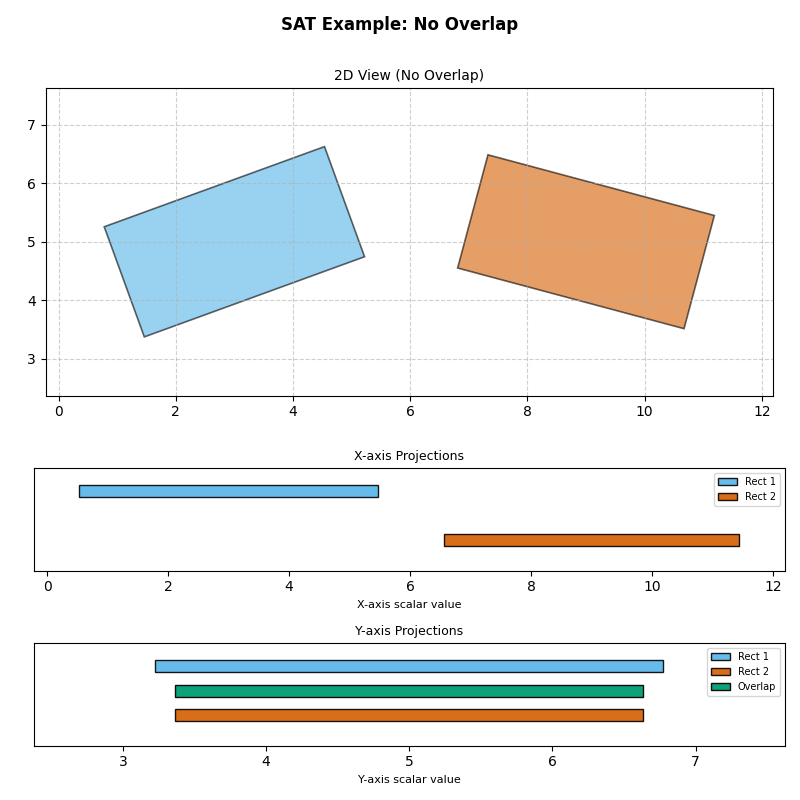
\includegraphics[width=\textwidth]{img/sat_no_overlap_colored.png}
		\caption{Separation Axis Theorem with no overlap}
		\label{fig:1a_sat}
	\end{subfigure}
	\hfill
	\begin{subfigure}{0.45\textwidth}
		\centering
		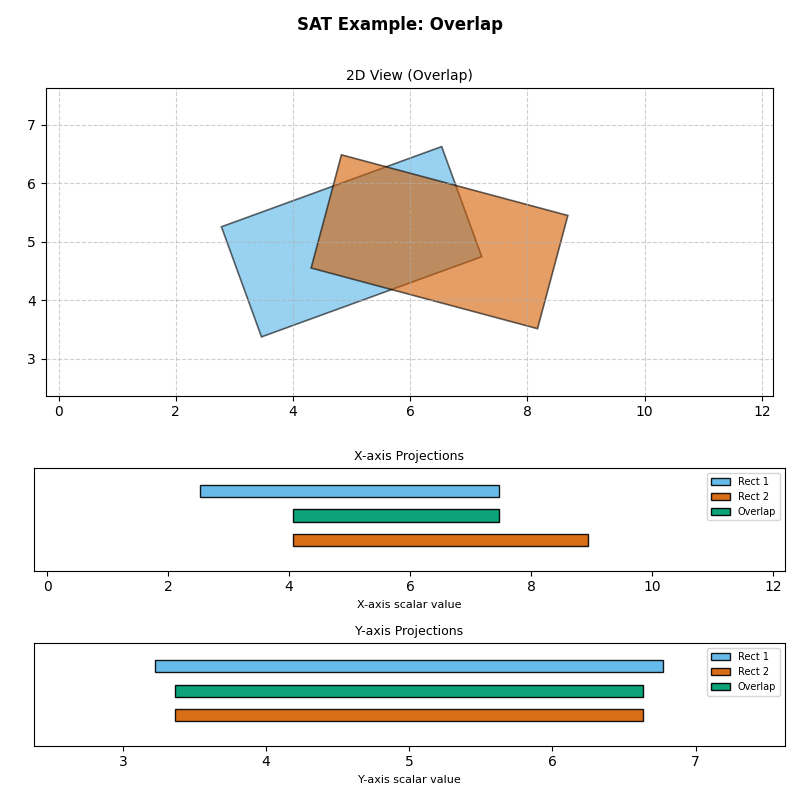
\includegraphics[width=\textwidth]{img/sat_overlap_colored.png}
		\caption{Separation Axis Theorem with overlap}
		\label{fig:1b_sat}
	\end{subfigure}
	
	\caption{Separation Axis Theorem for oriented rectangles. Each figure consists of three subplots. The first subplot illustrates the spatial configuration of the rectangles. The second and third subplots show the projections of their principal axes onto the $x$- and $y$-axes, respectively. An overlap occurs when the projections intersect along both axes; the overlap is highlighted in black in the second and third subplots.}
	\label{fig:sat_theorem}
\end{figure}

During the search phase (lines~\ref{alg:start_pso_update}--\ref{alg:end_pso_update} of Algorithm~\ref{alg:pso_fixtures}), the velocity matrix $V_s$ and the position matrix $P_s$ associated with particle $s$ are iteratively updated according to the standard PSO update equations.

Whenever possible, constraint violations arising from updated fixture positions are mitigated through dedicated geometric repair procedures, as reported in lines~\ref{alg:start_fixing_geom}--\ref{alg:end_fixing_geom} of Algorithm~\ref{alg:pso_fixtures}. For each fixture, if its geometry lies partially or entirely outside the workpiece boundary, the nearest vertex of the workpiece polygon and the fixture vertex farthest from it are identified. The fixture is then translated by the minimum displacement required to satisfy the boundary constraint. The repair strategy is limited to geometric violations, as these constraints are the most suitable for correction without adversely affecting the satisfaction of other constraints.

In lines~\ref{alg:start_fixing_type}--\ref{alg:end_fixing_type} of Algorithm~\ref{alg:pso_fixtures}  fixtures with type zero, representing unused fixtures, are assigned the dummy lower-left corner coordinates \((\wtab,\htab)\), as in the CP model formulation (see Section~\ref{sec:cp_cons}), and are excluded from constraint violation evaluations.

To guide the search toward constraint-respecting positions, as illustrated in lines~\ref{alg:start_deb_eval}--\ref{alg:end_deb_eval} of Algorithm~\ref{alg:pso_fixtures}, candidate solutions are evaluated using Deb’s rules~\cite{deb2000efficient}:
\begin{itemize}
	\item Between two feasible solutions, retain the one with the higher objective value.
	\item Between a feasible and an infeasible solution, retain the feasible one.
	\item Between two infeasible solutions, retain the one with the lower constraint violation.
\end{itemize}

After updating the personal best position $P^*_s$ of each particle $s$ using Deb’s rules, the global best position $P^*$ of the swarm is updated accordingly. At the end of the final iteration, the best position found by the swarm is returned.